\documentclass[a4paper,10pt,twocolumn]{ltjsarticle}
\usepackage[haranoaji]{luatexja-preset}
\usepackage[top=18mm,bottom=20mm,left=17mm,right=17mm,columnsep=8mm]{geometry}
\usepackage{graphicx,booktabs,array,caption,enumitem,xcolor,tikz}
\usetikzlibrary{shapes.geometric}
\setlength{\parindent}{1\zw}
\renewcommand{\baselinestretch}{1.0}
\setlength{\parskip}{0pt}
\renewcommand{\thesection}{\arabic{section}.}
\renewcommand{\thesubsection}{\arabic{section}.\arabic{subsection}.}
\makeatletter
\renewcommand{\section}{\@startsection{section}{1}{\z@}{1.1\Cvs \@plus.4\Cdp \@minus.2\Cdp}{.5\Cvs \@plus.2\Cdp}{\normalfont\gtfamily\bfseries\large}}
\renewcommand{\subsection}{\@startsection{subsection}{2}{\z@}{.8\Cvs \@plus.3\Cdp \@minus.2\Cdp}{.3\Cvs \@plus.1\Cdp}{\normalfont\gtfamily\bfseries\normalsize}}
\makeatother
\captionsetup{font={small,sf},labelsep=space,justification=raggedright,singlelinecheck=false,skip=3pt}
\captionsetup[table]{position=top}
\setlist[itemize]{leftmargin=1.2\zw,itemsep=0pt,topsep=2pt,parsep=0pt}
\setlength{\textfloatsep}{8pt plus 2pt minus 2pt}
\setlength{\floatsep}{8pt plus 2pt minus 2pt}
\setlength{\intextsep}{8pt plus 2pt minus 2pt}
\pagestyle{plain}
\raggedbottom
\begin{document}
\twocolumn[{
\noindent\fbox{\gtfamily\small\ 生成AI論文\ }\par\medskip
\begin{center}
{\gtfamily\bfseries\LARGE 得点の高い国ほど数学の男女差は小さいのか：PISA 2025の90の国・地域で確かめる$^{\dagger}$}\par\medskip
{\gtfamily\bfseries\large 数学的リテラシーの男女得点差と平均得点の水準の関連}\par\medskip
{\normalsize EduData調査研究グループ$^{*1}$・教育データサイエンス解析班$^{*2}$}\par
{\small オープン教育統計推進プロジェクト$^{*1}$・初等中等STEM教育データ基盤ユニット$^{*2}$}
\end{center}\smallskip
\noindent\begin{minipage}{\textwidth}\small 本研究は，OECDが公表したPISA 2025の表から，数学的リテラシーの男女得点差（男子−女子）を90の国・地域について整理し，平均得点の水準との関連を検討した．男子の得点が高い国・地域が71，女子が高い国・地域が19であった．標準誤差の1.96倍を超える差は，男子が高い国・地域で55，女子が高い国・地域で7であり，28の国・地域では偶然の範囲を超える差が見られなかった．平均得点が高い国・地域ほど男女差が小さいという予想に反し，平均得点と男女得点差の間には弱い正の相関が見られた（\textit{r}=.31，\textit{BF}\textsubscript{10}=5.91）．日本は平均得点が525.4点で5番目，男女得点差は16.3点（標準誤差5.7）で90の国・地域のうち19番目に大きかった．得点の上位に偏った7か国（基準の記録のない別の分析の対象国）だけを取り出すと逆向きの関連（\textit{r}=−.86）が得られ，国の選び方で結論が変わりうることも示した．これらは国・地域を単位とした集計値の関連であり，個々の生徒の因果や理由を示すものではない．\par\smallskip
\noindent{\gtfamily キーワード：}PISA 2025，数学的リテラシー，男女差，国際比較，生態学的誤謬\end{minipage}\medskip
}]
\let\thefootnote\relax
\footnotetext{\footnotesize 2026年10月執筆\\ $^{\dagger}$Is the Gender Gap in Mathematics Smaller in Higher-Performing Countries? Evidence from 90 Countries and Economies in PISA 2025\\ $^{*1}$ Open Education Data Project, Tokyo, Japan\quad $^{*2}$ Educational Data Science Unit, Tokyo, Japan}
\section{はじめに}
\subsection{研究の背景}
数学の得点に男女差があるかどうかは，長く論じられてきた．Hyde et al. (2008)は米国の州の学力調査を分析し，数学の男女差は小さいと報告した．Lindberg et al. (2010)は1990年から2007年の242の研究のメタ分析で，効果量が\textit{d}=.05と，男女差はほとんどないことを示した．一方，国による違いも報告されている．Else-Quest et al. (2010)は，TIMSSとPISAの2003年のデータを用いたメタ分析で，男女差の大きさが国によって異なり，男女平等に関する指標と関連することを報告した．Guiso et al. (2008)も，男女平等の度合いが高い国ほど数学の男女差が小さいことを示している．

ここから，「得点が高く，社会が成熟した国ほど男女差は小さいのではないか」という予想が生まれる．OECD (2026)が公表したPISA 2025（15歳の生徒の調査，主要分野は科学で数学は副次的な分野）は，90の国・地域について，数学の男女別の平均得点と差の標準誤差を示している．この表で，予想が成り立つかを確かめることができる．
\subsection{リサーチクエスチョン}
本研究の目的は，PISA 2025の公表値を用いて，数学的リテラシーの男女得点差の分布と，平均得点の水準との関連を記述することである．次の2つの研究課題を置く．
\begin{itemize}
\item RQ1：数学の男女得点差（男子−女子）は，国・地域によってどう違うか．標準誤差を考慮して，男子または女子のほうが高いと言える国・地域はどれくらいあるか．日本はどこに位置するか．
\item RQ2：平均得点が高い国・地域ほど，男女得点差は小さいか．
\end{itemize}
\section{調査対象および分析方法}
OECDが公表したPISA 2025 Results (Volume I)の表から，数学的リテラシーの平均得点（男女計），男子と女子の平均得点，男女得点差（男子−女子）とその標準誤差を，国・地域ごとに取り込んだ．対象は90の国・地域で，OECD平均は含めない．ウズベキスタンは公表値が欠けているため除いた．カナダ・アメリカなど6か国は，OECDの表で標本抽出基準についての注意がついている．

RQ1では，男女得点差が標準誤差の1.96倍を超える国・地域を，偶然の範囲を超える差（おおよそ5\%水準で有意）とみなした．国・地域ごとの比較を多数行うため，個々の判定は目安である．RQ2では，平均得点と男女得点差の関連をピアソンの積率相関係数 \textit{r} で示し，\textit{p} 値とJZSベイズファクター（\textit{BF}\textsubscript{10}），スピアマンの順位相関係数 \textit{ρ}，\textit{r} の95\%信頼区間（フィッシャーのz変換）を算出した．各国・地域を同じ重みで扱い，頑健性を確かめるため，特定の国・地域を除いた場合，男女得点差の標準誤差の逆数の2乗で重みをつけた場合，ブートストラップによる信頼区間も調べた．個々の判定の多重比較には，HolmとBenjamini-Hochbergの補正を用いた．分析単位は国・地域であり，個票は用いていない．

7か国だけの分析は，付随的な探索である．この7か国（日本，シンガポール，韓国，エストニア，カナダ，イギリス，アメリカ）は，本研究のために選んだのではなく，本プロジェクトの別の分析（PISAの7か国とOECD平均の経年比較）があらかじめ対象にしている国である．その選定の基準は記録に残っておらず，ここでは理由を示せない．90の国・地域の結果を見たあとに，同じ国だけを取り出して相関を計算したので，事前に決めた検定ではなく，事後の探索である．7か国はいずれも平均得点が上位27位以内（6か国は上位11位以内）にあり，7か国の平均得点（507.7点）は，90の国・地域の平均（428.9点）より高い．
\begin{table*}[!t]
\caption{主要指標の基本記述統計量}
\centering\small
\begin{tabular}{>{\raggedright\arraybackslash}p{9.2cm}rrrrrr}
\toprule
指標 & \textit{K} & 平均 & \textit{SD} & 中央値 & 最小 & 最大 \\
\midrule
数学得点 & 90 & 428.9 & 59.6 & 427.4 & 311.6 & 612.4 \\
男子得点 & 90 & 433.0 & 61.1 & 430.9 & 321.1 & 622.4 \\
女子得点 & 90 & 424.9 & 58.3 & 424.9 & 301.7 & 601.6 \\
男女得点差 & 90 & 8.0 & 9.3 & 9.1 & -27.2 & 24.0 \\
\bottomrule
\end{tabular}
\par\smallskip{\footnotesize 注）単位は点，\textit{K}は観測数（国・地域・区分）．}
\end{table*}
\begin{table*}[!t]
\caption{主要指標間のピアソンの相関係数と，ベイズファクター}
\centering\small
\begin{tabular}{>{\raggedright\arraybackslash}p{6.4cm}>{\raggedright\arraybackslash}p{6.4cm}rrr}
\toprule
指標 \textit{X} & 指標 \textit{Y} & \textit{r} & \textit{p} & \textit{BF}\textsubscript{10} \\
\midrule
数学得点 & 男女得点差 & .31 & = .003 & 5.91 \\
\bottomrule
\end{tabular}
\par\smallskip{\footnotesize 注）\textit{BF}\textsubscript{10}はJZSベイズファクター（3を超えれば関連を支持，1/3を下回れば関連がないことを支持）．全ペアの探索の一部を載せた．}
\end{table*}
\section{結果}
RQ1について，男女得点差の平均は8.0点（中央値は約9点）で，男子の得点が高い国・地域が71，女子が高い国・地域が19であった．標準誤差の1.96倍を超える差が見られたのは，男子が高い国・地域で55，女子が高い国・地域で7（パレスチナ，ブルガリア，モンゴル，マルタ，タイ，フィリピン，インドネシア）で，残る28の国・地域では偶然の範囲を超える差は見られなかった．90の判定に多重比較の補正（Holm）を行うと，差が認められるのは44（男子が高い41，女子が高い3），Benjamini-Hochbergの補正では60（男子が高い53，女子が高い7）であった．男子が高い差が大きいのは，イギリス（24.0点），アメリカ（23.8点），ルワンダ（23.0点），オーストリア（22.7点），コスタリカ（22.3点）であり，女子が高い差が最も大きいのはパレスチナ（−27.2点）であった．

RQ2について，平均得点と男女得点差の間には，弱い正の相関が見られた（\textit{r}=.31，95\%CI [.10, .48]，\textit{ρ}=.33，\textit{n}=90，\textit{p}=.003，\textit{BF}\textsubscript{10}=5.91）．すなわち，平均得点が高い国・地域ほど，男女得点差が小さいのではなく，むしろ大きい傾向があった．平均得点で90の国・地域を30ずつに分けると，男女得点差の平均は，低い群で6.7点，中ほどの群で3.8点，高い群で13.6点であり，直線的ではなかった．平均得点の上位30の国・地域だけで見ると，関連はほとんどなかった（\textit{r}=.10，\textit{p}=.59）．関連は特定の国・地域に依存していなかった．平均得点の上位3地域（北京・上海・江蘇・浙江，シンガポール，マカオ）を除くと \textit{r}=.26，上位4地域（台湾を加える）を除くと \textit{r}=.29で，関連は弱まるが正のままであり，標本抽出基準の注意がある6か国を除いても \textit{r}=.29，1か国ずつ除いた場合の範囲は .28〜.35，標準誤差で重みをつけると \textit{r}=.33，ブートストラップの95\%信頼区間は [.10, .49] であった．説明される分散は約9\%（\textit{r}\textsuperscript{2}=.09）にとどまる．平均得点が高い国・地域の男女得点差は，北京・上海・江蘇・浙江（612.4点）で20.8点，シンガポール（562.9点）で9.8点，マカオ（549.3点）で18.5点，台湾（546.2点）で1.3点，韓国（522.3点）で10.9点と，ばらつきが大きかった．

日本は，平均得点が525.4点で5番目に高く，男女得点差は16.3点（標準誤差5.7）で，90の国・地域のうち19番目に大きかった．この差は標準誤差の1.96倍（11.2点）を超えており，男子が高いと言える範囲にある．なお，別の分析が主要国として使っている日本・シンガポール・韓国・エストニア・カナダ・イギリス・アメリカの7か国だけを取り出して（選定の経緯は方法に記した），同じ関連を見ると，\textit{r}=−.86（\textit{n}=7，\textit{p}=.012）と逆向きになった．90の国・地域から無作為に7つを選ぶ操作を5,000回繰り返すと，\textit{r} が −.86以下になったのは0.1\%にすぎず，負の相関になったのは約2割であった．
\begin{figure}[t]\centering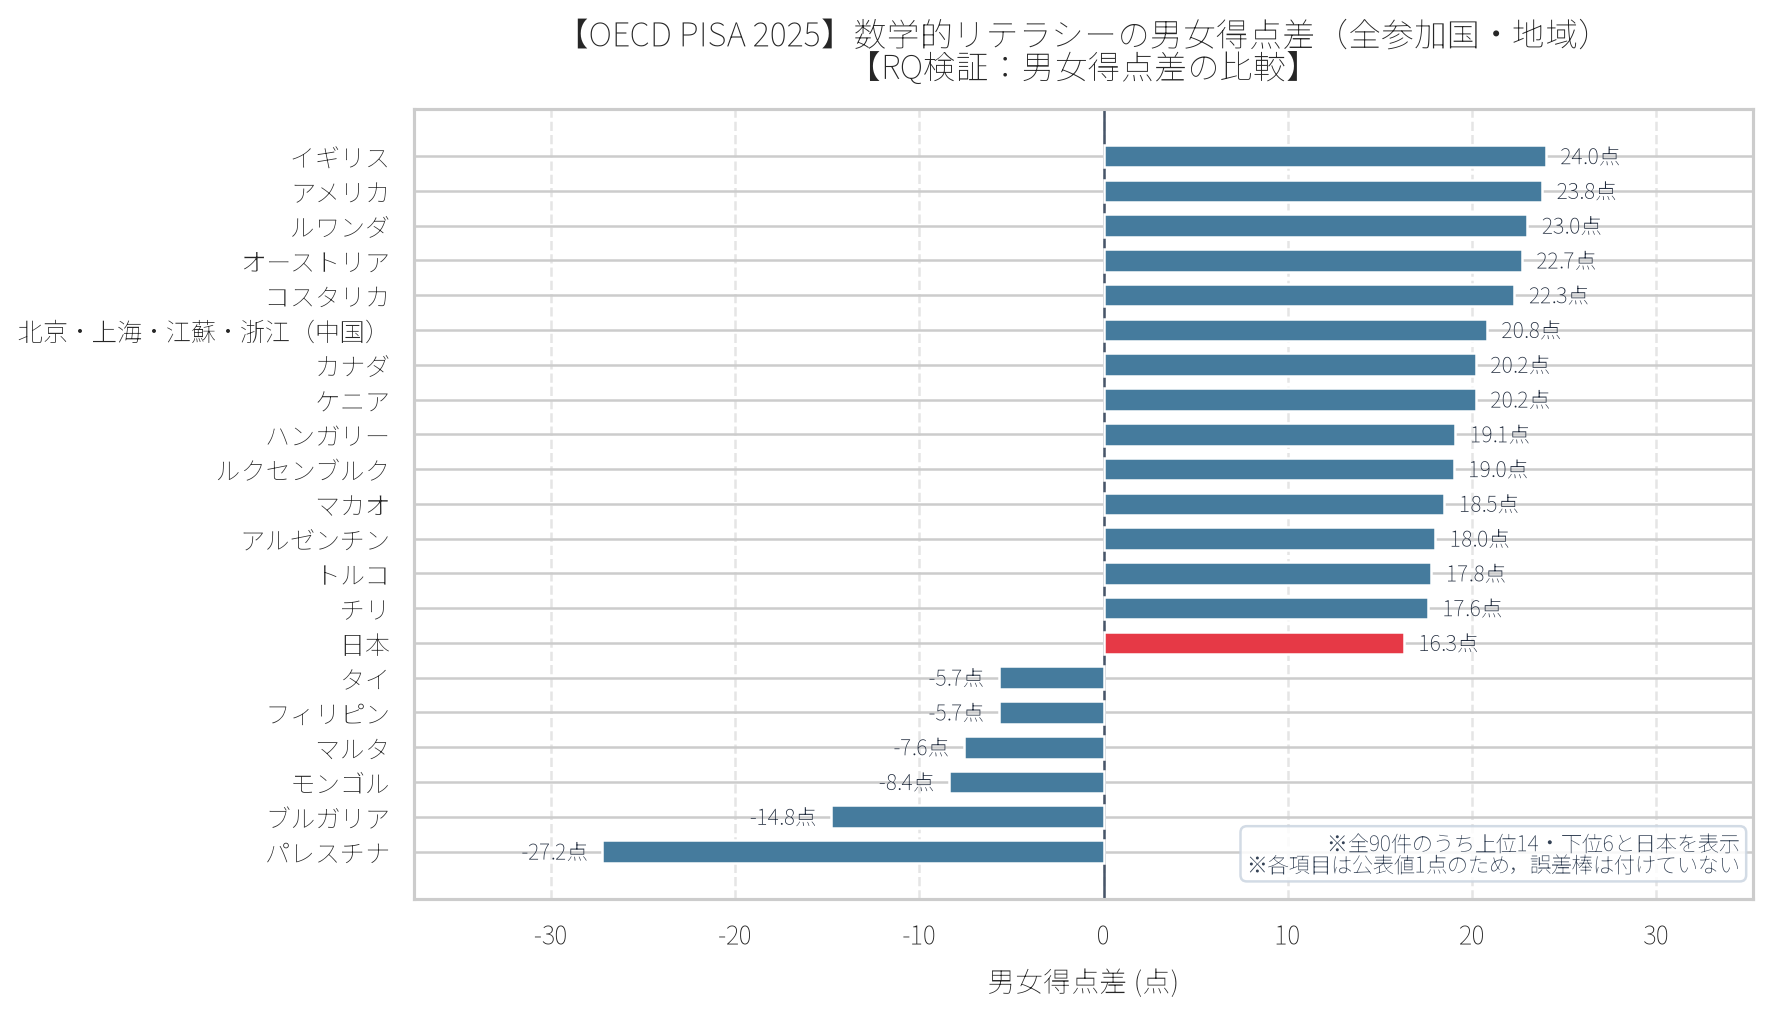
\includegraphics[width=\columnwidth]{chart_oecd_pisa2025_gender_gap.png}\caption{男女得点差の値の比較（上位・下位と日本を抜粋）．赤が日本}\end{figure}
\begin{figure}[t]\centering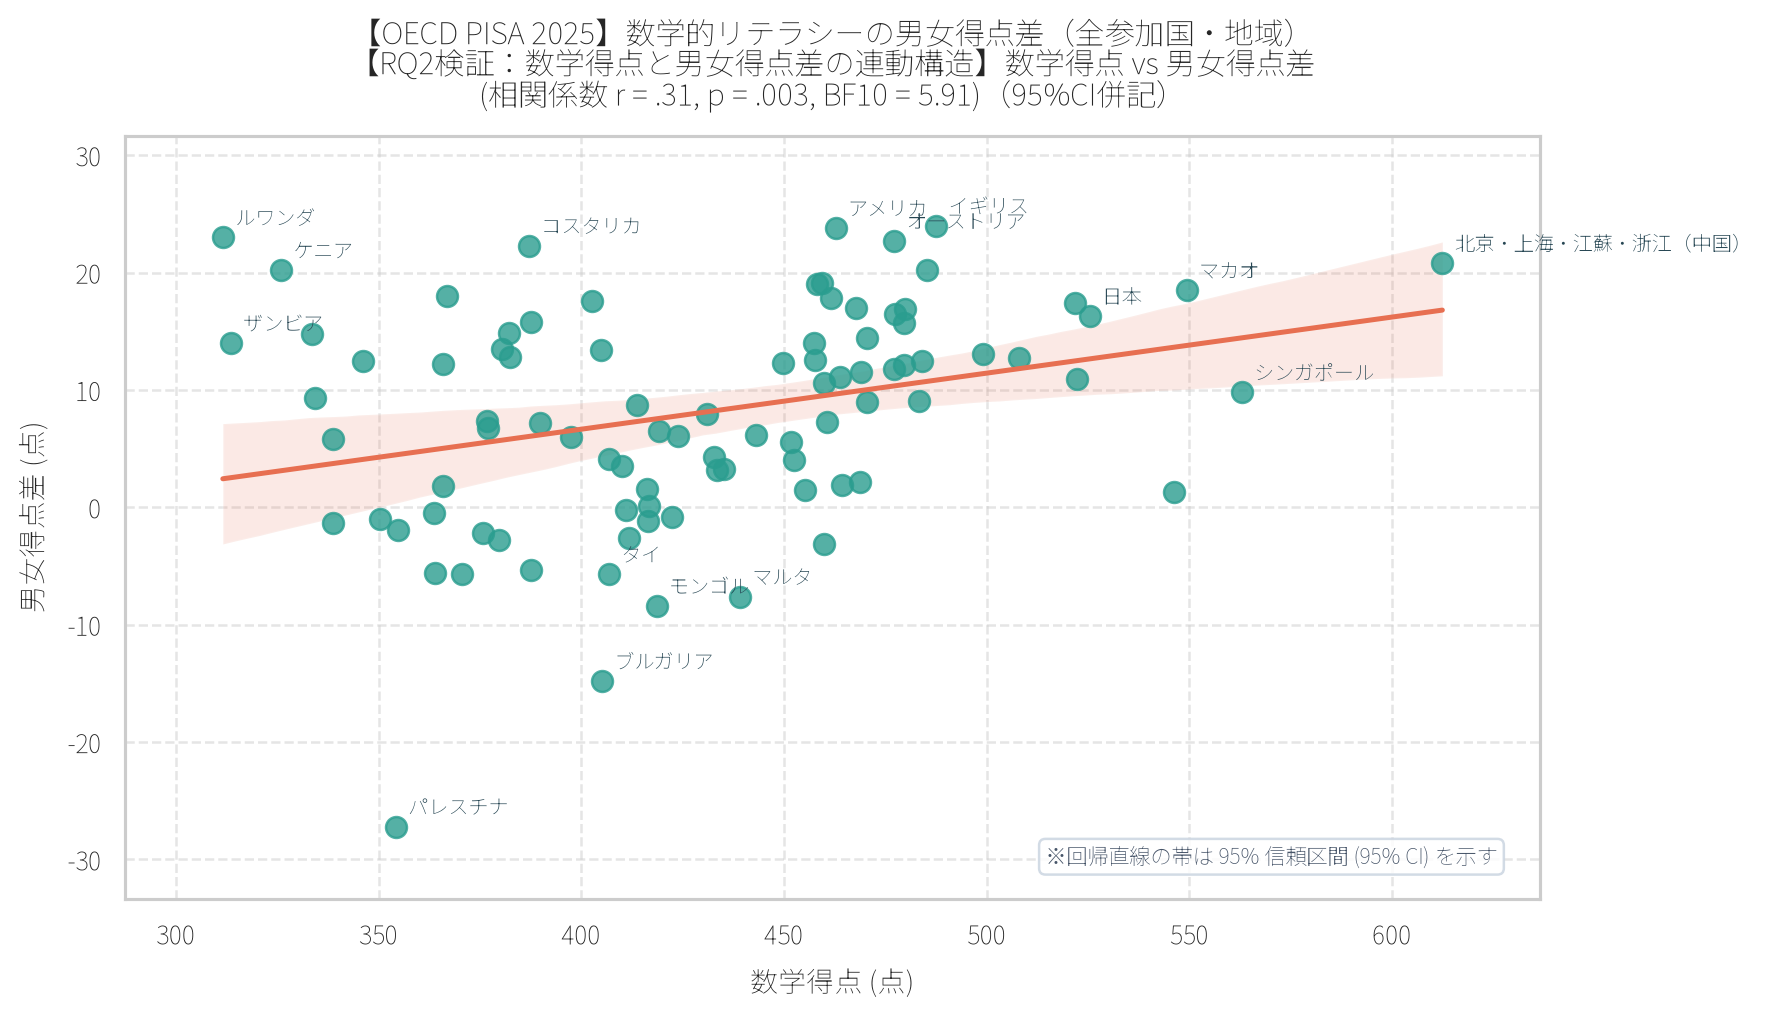
\includegraphics[width=\columnwidth]{chart_secondary_oecd_pisa2025_gender_gap.png}\caption{数学得点と男女得点差の関連（回帰直線と，その平均の95\%信頼区間の帯，n=90）}\end{figure}
\section{考察}
RQ1とRQ2の結果をまとめると，PISA 2025の数学では，90の国・地域のうち71で男子の得点が高く，その多くで差は標準誤差を超えていた．一方，女子が高い国・地域も19あり，差が標準誤差を超えない国・地域も28あった．この点で，男女差が国によって大きく異なるというElse-Quest et al. (2010)の報告と整合する．男女差が全体として小さいとするLindberg et al. (2010)やHyde et al. (2008)の知見とは，直接比べることができない．それらは効果量（標準偏差で割った差）で報告されたのに対し，本研究が使った表には得点の標準偏差がなく，効果量を計算していないためである．

平均得点が高い国・地域ほど男女差が小さいという予想は，90の国・地域では支持されなかった．Guiso et al. (2008)が男女平等の度合いと男女差の関連を示したことを踏まえると，平均得点の水準は，男女平等の度合いの代わりにはならないとみられる．ただし，本稿のデータには男女平等の指標がなく，その検討はしていない．また，7か国だけを選ぶと，逆向きの強い関連（\textit{r}=−.86）が得られた．無作為に7か国を選んでここまで強い負の相関になるのは稀であり，この7か国は，選定の基準が記録になく，得点の高い国・地域に偏っている（上位27位以内）．得点の範囲が狭いことも含め，7か国という選び方が結果を左右した可能性がある．国の数が少ないと，どの国を含めるかで関連の向きまで変わる．この関連の理由は，本研究のデータでは検証できない．ステレオタイプ脅威（Spencer et al., 1999）のような心理的要因や，数学・理系をめぐる複数の要因（Blickenstaff, 2005）が論じられてきたが，本稿にはこれらを測った変数がない．

日本は得点が高く，男女得点差も標準誤差を超えて男子が高い位置にある．これを授業や制度のあり方の帰結と読むことはできない．OECD (2023)が示したPISA 2022の結果との比較や，同じ生徒の変化は，本稿の範囲を超える．本研究の限界は，(1)国・地域の集計値のみを用いており個人の因果を特定できないこと，(2)男女平等や経済水準などを統制していないこと，(3)標準誤差にもとづく判定を多数回行っており，補正を行うと差が認められる国・地域の数が減ること，(4)6か国の標本抽出基準についての注意を考慮していないこと，である．今後は，男女平等の指標を加えた分析と，個票を用いた個人レベルの分析が必要である．
\section*{参考文献}
\begingroup\scriptsize\raggedright\interlinepenalty=10000 
\begin{list}{}{\setlength{\leftmargin}{1.5\zw}\setlength{\itemindent}{-1.5\zw}\setlength{\labelwidth}{0pt}\setlength{\labelsep}{0pt}\setlength{\itemsep}{1pt}\setlength{\parsep}{0pt}\setlength{\topsep}{0pt}\setlength{\listparindent}{0pt}}
\item BLICKENSTAFF, J. C. (2005) Women and science careers: Leaky pipeline or gender filter? Gender and Education, \textbf{17} (4) ：369-386.
\item ELSE-QUEST, N. M., HYDE, J. S. and LINN, M. C. (2010) Cross-national patterns of gender differences in mathematics: A meta-analysis. Psychological Bulletin, \textbf{136} (1) ：103-127.
\item GUISO, L., MONTE, F., SAPIENZA, P. and ZINGALES, L. (2008) Culture, gender, and math. Science, \textbf{320} (5880) ：1164-1165.
\item HYDE, J. S., LINDBERG, S. M., LINN, M. C., ELLIS, A. B. and WILLIAMS, C. C. (2008) Gender similarities characterize math performance. Science, \textbf{321} (5888) ：494-495.
\item LINDBERG, S. M., HYDE, J. S., PETERSEN, J. L. and LINN, M. C. (2010) New trends in gender and mathematics performance: A meta-analysis. Psychological Bulletin, \textbf{136} (6) ：1123-1135.
\item OECD (2023) PISA 2022 Results (Volume I): The State of Learning and Equity in Education. OECD Publishing, Paris. DOI: 10.1787/53f23881-en
\item OECD (2026) PISA 2025 Results (Volume I). OECD Publishing, Paris. DOI: 10.1787/73451bc5-en
\item SPENCER, S. J., STEELE, C. M. and QUINN, D. M. (1999) Stereotype threat and women's math performance. Journal of Experimental Social Psychology, \textbf{35} (1) ：4-28.
\end{list}\endgroup
\section*{Summary}
{\footnotesize\setlength{\parindent}{0pt}Using the published PISA 2025 tables, we described the gender gap in mathematics performance (boys minus girls) in 90 countries and economies and examined its relation to mean performance. Boys outperformed girls in 71 countries or economies and girls outperformed boys in 19. A gap larger than 1.96 standard errors was found in 55 countries where boys scored higher and in 7 where girls scored higher; in 28 no gap beyond chance was found. Contrary to the expectation that higher-performing countries have smaller gaps, mean performance and the gap were weakly and positively correlated (r = .31, BF10 = 5.91). Japan ranked 5th in mean performance (525.4) and 19th in the size of the gap (16.3 points, SE 5.7). A post hoc analysis of seven countries alone, all within the top 27 in mean performance and taken from another analysis in this project whose selection criteria are not recorded, gave the opposite sign (r = −.86), showing that the conclusion can depend on which countries are chosen. These are associations between country-level aggregates and do not show causation among individual students.\par\smallskip KEYWORDS: PISA 2025, MATHEMATICS, GENDER GAP, CROSS-COUNTRY, ECOLOGICAL FALLACY\par}
\medskip\noindent\fbox{\parbox{\dimexpr\columnwidth-2\fboxsep-2\fboxrule}{\footnotesize\gtfamily 【付記：生成AIによる自動執筆に関する開示】\\ 本論文は学生への教育目的で作成している．使用しているデータは公的オープンデータである．統計の算出はPythonで行い，文章は生成AI（Anthropic Claude等）を活用して作成した．記載した統計数値は元データに準拠しているが，教育学的な考察や提言の妥当性は，指導現場の実情に応じて，批判的に吟味してほしい．}}
\end{document}
